\section*{Ejercicio \#3}
A continuación se presenta una comparación del tiempo de procesamiento de cada algoritmo de ordenamiento por cada lenguaje de programación.
\subsection*{BubbleSort}
% Kem
\subsection*{CountingSort}
% Kem
\subsection*{HeapSort}
\subsection*{InsertionSort}
\subsection*{MergeSort}
\subsection*{QuickSort}
\subsection*{SelectionSort}

\subsection*{Todos los algoritmos de ordenamiento}
A continuación se muestra el desenvolvimiento de todos los algoritmos de ordenamiento implementado en un sólo lenguaje de programación: Ya sea \verb!C++!, \verb!Python! o \verb!Java!.
\begin{itemize}
    \item \textbf{C++}
    \item \textbf{Python}
    \item \textbf{Java}
        \begin{figure}[H]
	        \centering
	        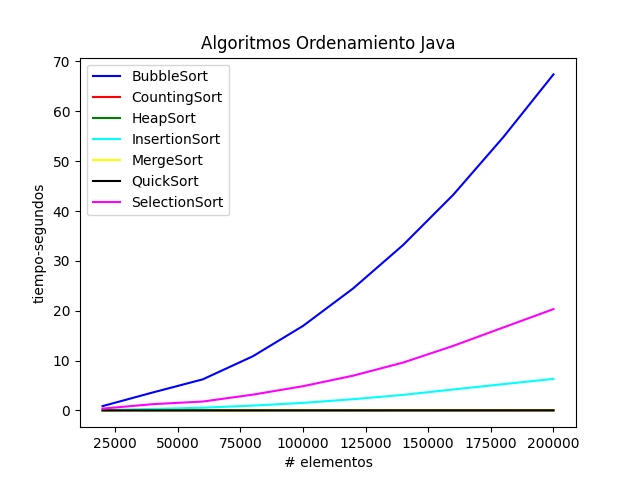
\includegraphics[scale=0.5]{../images/plots/Sorts_Java.png}
	        \caption{Gráfica de los algoritmos de ordenamiento implementados en Java, evaluando de 20000 hasta 200000 datos}
		\end{figure}
En la gráfica se aprecia que el algoritmo más lento para ordenar un array es el Bubble Sort, seguido del Selection Sort y el Insertion Sort.
        \begin{figure}[H]
	        \centering
	        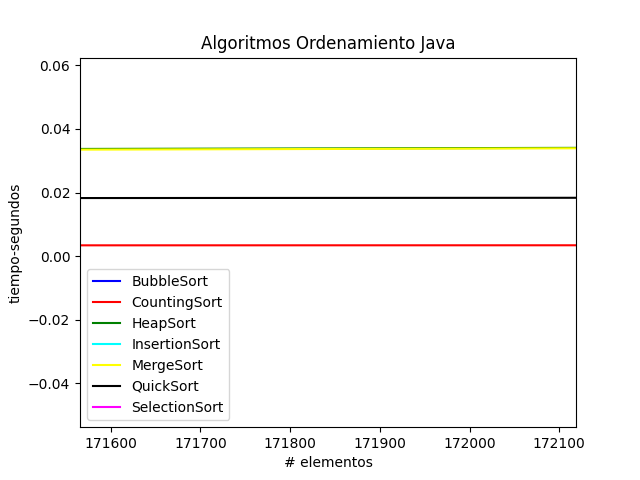
\includegraphics[scale=0.5]{Practica01/images/plots/Sorts2_Java.png}
	        \caption{Gráfica con acercamiento de los algoritmos de ordenamiento implementados en Java, evaluando de 100000 hasta 200000 datos}
		\end{figure}
En la gráfica con acercamiento se aprecia que el algoritmo más eficiente para ordenar un array es el Counting Sort, seguido del Quick Sort, el Merge Sort y el Heap Sort.
\end{itemize}

\iffalse
% ---- Para poner dos imágenes (una a lado de otra) ----
Como se muestra en la figuras \ref{fig:act-1_a} y \ref{fig:act-1_b}.
\begin{figure}[H]
\centering
\begin{minipage}{0.45\textwidth}
  \centering
  \includegraphics[width=0.9\textwidth]{act-1_a}
  \caption{Envío de \textit{ICMP ECHO REQUEST} de PC0 a PC1, PC2 y PC3.}
  \label{fig:act-1_a}
\end{minipage}\hfill
\begin{minipage}{0.45\textwidth}
  \centering
  \includegraphics[width=0.9\textwidth]{act-1_b}
  \caption{Respuesta de PC1, PC2 y PC3. Tabla ARP de PC0.}
  \label{fig:act-1_b}
\end{minipage}
\end{figure}
% ---- Para colocar una imagen ----
Como se muestra en la figura \ref{fig:act-3}
\begin{figure}[H]
  \centering
  \includegraphics[width=0.8\textwidth]{act-3}
  \caption{Tabla de subneteo para la red 192.168.100.0.}
  \label{fig:act-3}
\end{figure}
\fi